%  The AAU Poster Theme.
%  2013-05-08 v. 1.1.0
%  Copyright 2013 by Jesper Kjær Nielsen <jkn@es.aau.dk>
%
%  This is free software: you can redistribute it and/or modify
%  it under the terms of the GNU General Public License as published by
%  the Free Software Foundation, either version 3 of the License, or
%  (at your option) any later version.
%
%  This is distributed in the hope that it will be useful,
%  but WITHOUT ANY WARRANTY; without even the implied warranty of
%  MERCHANTABILITY or FITNESS FOR A PARTICULAR PURPOSE.  See the
%  GNU General Public License for more details.
%
%  You can find the GNU General Public License at <http://www.gnu.org/licenses/>.
%%%%%%%%%%%5\documentclass[paperwidth=24in,paperheight=48in, fontscale=0.4166666666666, landscape]{baposter}
\documentclass[paperwidth=24in,paperheight=48in, fontscale=0.4166666666666]{baposter}
%%%%%%%%%%%%%%%%%%%%%%%%%%%%%%%%%%%%%%%%%%%%%%%%
% Language, Encoding and Fonts
% http://en.wikibooks.org/wiki/LaTeX/Internationalization
%%%%%%%%%%%%%%%%%%%%%%%%%%%%%%%%%%%%%%%%%%%%%%%%
% Select encoding of your inputs. Depends on
% your operating system and its default input
% encoding. Typically, you should use
%   Linux  : utf8 (most modern Linux distributions)
%            latin1 
%   Windows: ansinew
%            latin1 (works in most cases)
%   Mac    : applemac
% Notice that you can manually change the input
% encoding of your files by selecting "save as"
% an select the desired input encoding. 
\usepackage[utf8]{inputenc}
% Make latex understand and use the typographic
% rules of the language used in the document.
\usepackage[english]{babel}
% Use the vector font Latin Modern which is going
% to be the default font in latex in the future.
\usepackage{helvet}
% Change the default font family from roman to sans serif
\renewcommand{\familydefault}{\sfdefault} % for text
\usepackage[helvet]{sfmath} % for math
% Choose the font encoding
\usepackage[T1]{fontenc}

%%%%%%%%%%%%%%%%%%%%%%%%%%%%%%%%%%%%%%%%%%%%%%%%
% Graphics and Tables
% http://en.wikibooks.org/wiki/LaTeX/Importing_Graphics
% http://en.wikibooks.org/wiki/LaTeX/Tables
% http://pgfplots.sourceforge.net/
%%%%%%%%%%%%%%%%%%%%%%%%%%%%%%%%%%%%%%%%%%%%%%%%
% You cannot use floats in the baposter theme.
% We therefore load the caption package which provides
% the command \captionof
% Set up how figure and table captions are displayed
\usepackage{caption}
\captionsetup{
  font=small,% set font size to footnotesize
  labelfont=bf % bold label (e.g., Figure 3.2) font
}
% Make the standard latex tables look so much better
\usepackage{array,booktabs}

%%%%%%%%%%%%%%%%%%%%%%%%%%%%%%%%%%%%%%%%%%%%%%%%
% Mathematics
% http://en.wikibooks.org/wiki/LaTeX/Mathematics
%%%%%%%%%%%%%%%%%%%%%%%%%%%%%%%%%%%%%%%%%%%%%%%%
% Defines new environments such as equation,
% align and split 
\usepackage{amsmath}
% Adds new math symbols
\usepackage{amssymb}

%%%%%%%%%%%%%%%%%%%%%%%%%%%%%%%%%%%%%%%%%%%%%%%%
% Colours
% http://en.wikibooks.org/wiki/LaTeX/Colors
%%%%%%%%%%%%%%%%%%%%%%%%%%%%%%%%%%%%%%%%%%%%%%%%
\selectcolormodel{RGB}
% define the three aau colors
\definecolor{aaublue1}{RGB}{161,0,0}% dark blue
\definecolor{aaublue2}{RGB}{228,63,41} % light blue
\definecolor{aaublue3}{RGB}{194, 182, 170}%{194,182,158}%{194,193,204} % lighter blue
\definecolor{blackcolor}{RGB}{10,10,10}

%%%%%%%%%%%%%%%%%%%%%%%%%%%%%%%%%%%%%%%%%%%%%%%%
% Lists
% http://en.wikibooks.org/wiki/LaTeX/List_Structures
%%%%%%%%%%%%%%%%%%%%%%%%%%%%%%%%%%%%%%%%%%%%%%%%
% Easier configuration of lists
\usepackage{enumitem}
%configure itemize
\setlist{%
  topsep=0pt,% set space before and after list
  noitemsep,% remove space between items
  labelindent=\parindent,% set the label indentation to the paragraph indentation
  leftmargin=*,% remove the left margin
  font=\color{aaublue1}\normalfont, %set the colour of all bullets, numbers and descriptions to aaublue1
}


\usepackage{pifont}

\newcommand*{\pd}[2]{\ensuremath{\dfrac{\partial #1}{\partial #2}}}
\newcommand*{\inpd}[2]{\ensuremath{\frac{\partial #1}{\partial #2}}}


% use set<itemize,enumerate,description> if you have an older latex distribution
\setitemize[1]{label={\raise1.25pt\hbox{$\blacktriangleright$}}}
\setitemize[2]{label={\scriptsize\raise1.25pt\hbox{$\blacktriangleright$}}}
\setitemize[3]{label={\raise1.25pt\hbox{$\star$}}}
\setitemize[4]{label={-}}
%\setenumerate[1]{label={\theenumi.}}
%\setenumerate[2]{label={(\theenumii)}}
%\setenumerate[3]{label={\theenumiii.}}
%\setenumerate[4]{label={\theenumiv.}}
%\setdescription{font=\color{aaublue1}\normalfont\bfseries}

% use setlist[<itemize,enumerate,description>,<level>] if you have a newer latex distribution
%\setlist[itemize,1]{label={\raise1.25pt\hbox{$\blacktriangleright$}}}
%\setlist[itemize,2]{label={\scriptsize\raise1.25pt\hbox{$\blacktriangleright$}}}
%\setlist[itemize,3]{label={\raise1.25pt\hbox{$\star$}}}
%\setlist[itemize,4]{label={-}}
%\setlist[enumerate,1]{label={\theenumi.}}
%\setlist[enumerate,2]{label={(\theenumii)}}
%\setlist[enumerate,3]{label={\theenumiii.}}
%\setlist[enumerate,4]{label={\theenumiv.}}
%\setlist[description]{font=\color{aaublue1}\normalfont\bfseries}

%%%%%%%%%%%%%%%%%%%%%%%%%%%%%%%%%%%%%%%%%%%%%%%%
% Misc
%%%%%%%%%%%%%%%%%%%%%%%%%%%%%%%%%%%%%%%%%%%%%%%%
% change/remove some names
\addto{\captionsenglish}{
  %remove the title of the bibliograhpy
  \renewcommand{\refname}{\vspace{-0.7em}}
  %change Figure to Fig. in figure captions
  \renewcommand{\figurename}{Fig.}
}
% create links
\usepackage{url}
%note that the hyperref package is currently incompatible with the baposter class

%%%%%%%%%%%%%%%%%%%%%%%%%%%%%%%%%%%%%%%%%%%%%%%%
% Macros
%%%%%%%%%%%%%%%%%%%%%%%%%%%%%%%%%%%%%%%%%%%%%%%%
\newcommand{\alert}[1]{{\color{aaublue1}#1}}

%%%%%%%%%%%%%%%%%%%%%%%%%%%%%%%%%%%%%%%%%%%%%%%%
% Document Start 
%%%%%%%%%%%%%%%%%%%%%%%%%%%%%%%%%%%%%%%%%%%%%%%%
\begin{document}
%%%%%%%%%%%%%%%%%%%%%%%%%%%%%%%%%%%%%%%%%%%%%%%%
% Some changes that cannot be made in the preamble
%%%%%%%%%%%%%%%%%%%%%%%%%%%%%%%%%%%%%%%%%%%%%%%%
% set the background of the poster
\background{
  \begin{tikzpicture}[remember picture,overlay]%
    %the poster background color
    \fill[fill=aaublue3] (current page.north west) rectangle (current page.south east);
    %the header
    \fill [fill=aaublue1] (current page.north west) rectangle ([yshift=-\headerheight] current page.north east);
  \end{tikzpicture}
}
% if you want to reduce the space before and after equations, use and adjust
% the following lines
\addtolength{\abovedisplayskip}{-2mm}
\addtolength{\belowdisplayskip}{-2mm}

%%%%%%%%%%%%%%%%%%%%%%%%%%%%%%%%%%%%%%%%%%%%%%%%
% General poster setup
%%%%%%%%%%%%%%%%%%%%%%%%%%%%%%%%%%%%%%%%%%%%%%%%
\begin{poster}{
  %general options for the poster
  grid=false,
  columns=2,
%  colspacing=4.2mm,
  headerheight=0.027\textheight,
  background=user,
%  bgColorOne=red!42, %is used when background != user and none
%  bgColortwo=green!42, %is used when background is shaded
  eyecatcher=true,
  %posterbox options
  headerborder=closed,
  borderColor=aaublue1,
  headershape=rectangle,
  headershade=plain,
  headerColorOne=aaublue1,
%  headerColortwo=yellow!42, %is used when the header background is shaded
  textborder=rectangle,
  boxshade=plain,
  boxColorOne=white,
%  boxColorTwo=cyan!42,%is used when the text background is shaded
  headerFontColor=white,
  headerfont=\Large\sf\bf,
  linewidth=3pt
}
%the Eye Catcher (the logo on the left)
{
  %this can be commented out or replaced by a company/department logo
  %%%%%%5
\includegraphics[height=0.75\headerheight]{aau_logo_new_neg}
}
%the poster title
{\color{white}\bf
\vspace{12pt}
  Dense Face Detection
}
%the author(s)
%%%{\color{white}\small
%%%  \vspace{1em} Jesper Kjær Nielsen\\[0.5em]
%%%  Dept.\ of Electronic Systems, Aalborg University, Denmark\\
%%%  jkn@es.aau.dk
%%%}
%the logo (the logo on the right)
{
  %this can be commented out or replaced by a company/department logo
  %%%%%%%5
\includegraphics[height=0.75\headerheight]{aau_logo_new_neg}
}

%%%%%%%%%%%%%%%%%%%%%%%%%%%%%%%%%%%%%%%%%%%%%%%%
% the actual content of the poster begins here
%%%%%%%%%%%%%%%%%%%%%%%%%%%%%%%%%%%%%%%%%%%%%%%%

\begin{posterbox}[name=intro,column=0,row=0]{Introduction and Rationale}
\scalebox{0.00000000000000000001}{
\begin{minipage}{0.0001\linewidth}
  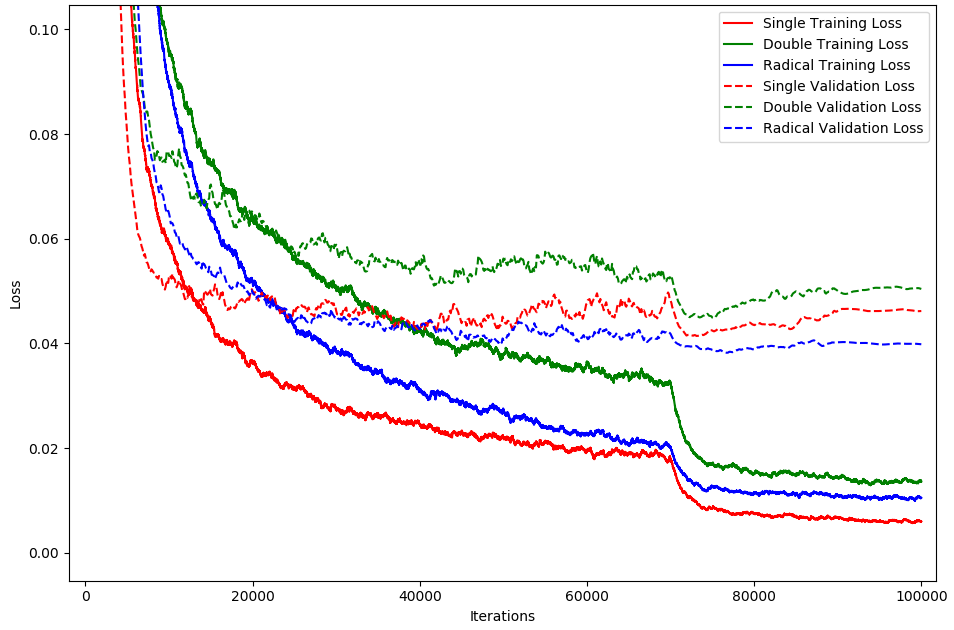
\includegraphics[width=0.02cm]{seqmnistloss.png}
  \captionof{figure}{\footnotesize{SequenceMNIST training and validation losses}} 
\end{minipage}
\begin{minipage}{0.0001\linewidth}
  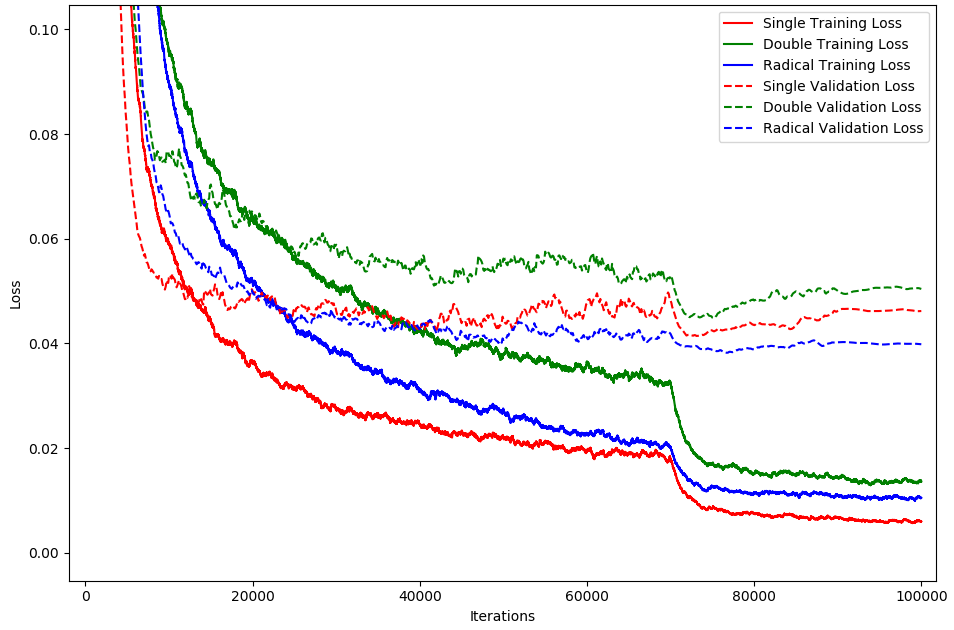
\includegraphics[width=0.02cm]{seqmnistloss.png}
  \captionof{figure}{\footnotesize{SequenceMNIST training and validation losses}} 
\end{minipage}
\begin{minipage}{0.0001\linewidth}
  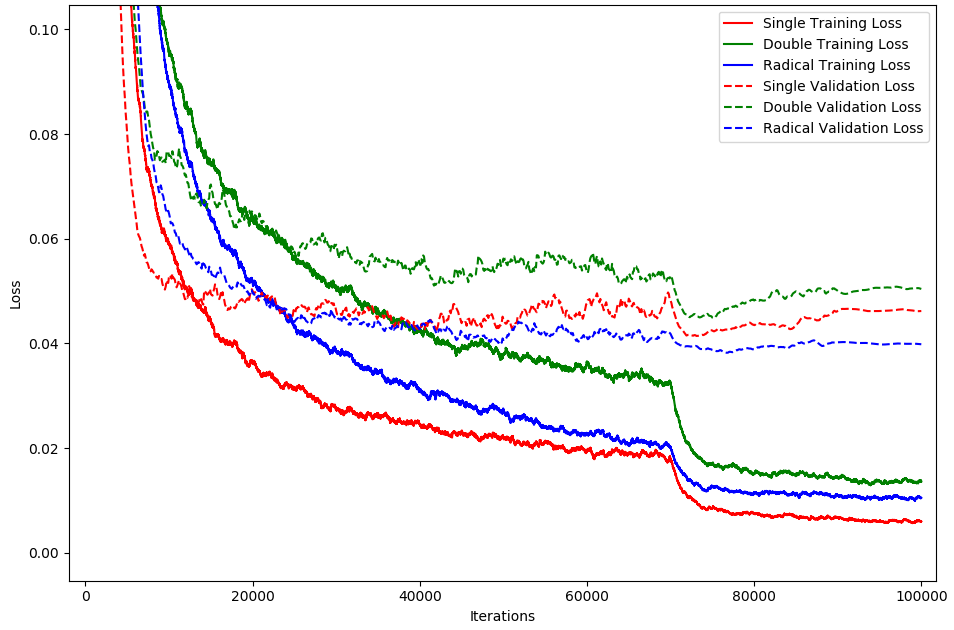
\includegraphics[width=0.02cm]{seqmnistloss.png}
  \captionof{figure}{\footnotesize{SequenceMNIST training and validation losses}} 
\end{minipage}
\begin{minipage}{0.0001\linewidth}
  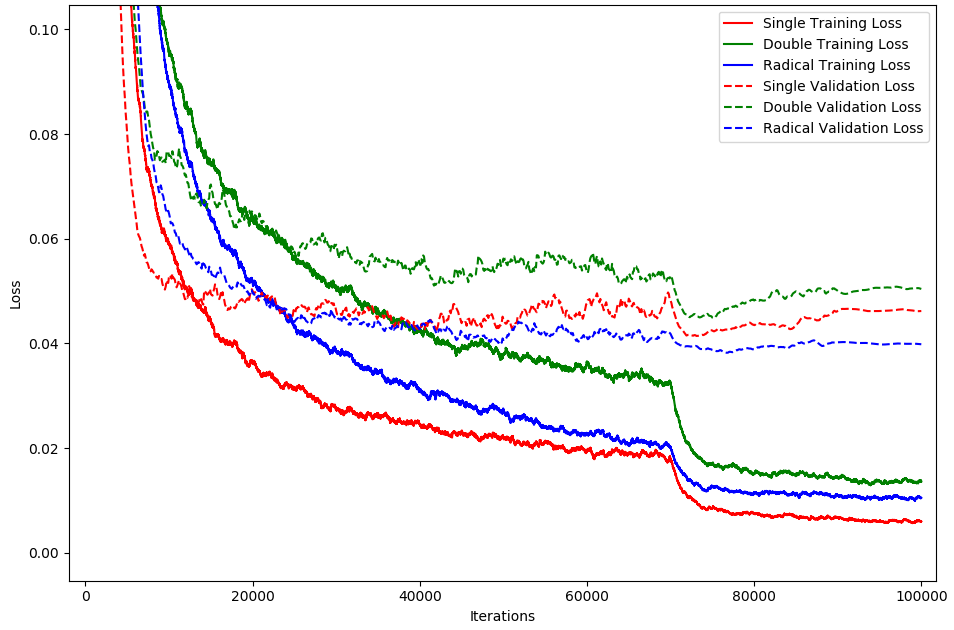
\includegraphics[width=0.02cm]{seqmnistloss.png}
  \captionof{figure}{\footnotesize{SequenceMNIST training and validation losses}} 
\end{minipage}
\begin{minipage}{0.0001\linewidth}
  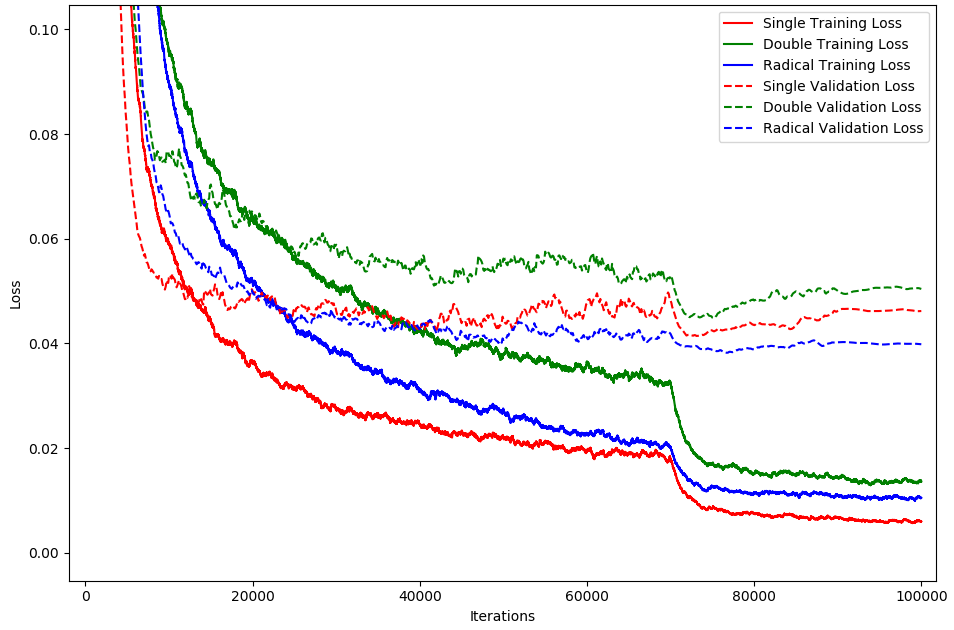
\includegraphics[width=0.02cm]{seqmnistloss.png}
  \captionof{figure}{\footnotesize{SequenceMNIST training and validation losses}} 
\end{minipage}
\begin{minipage}{0.0001\linewidth}
  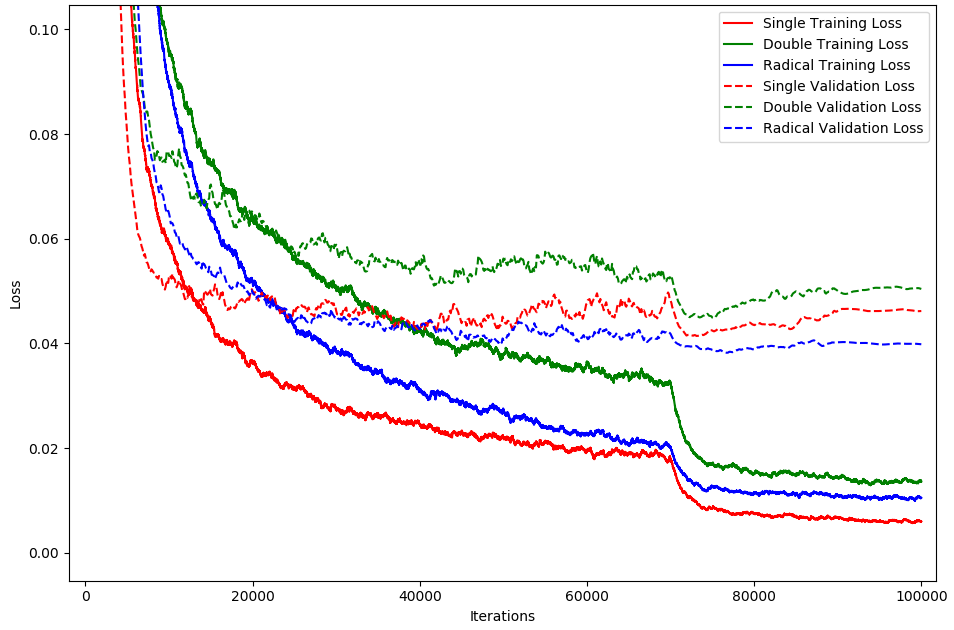
\includegraphics[width=0.02cm]{seqmnistloss.png}
  \captionof{figure}{\footnotesize{SequenceMNIST training and validation losses}} 
\end{minipage}
\begin{minipage}{0.7\linewidth}
   \centering
   \label{tabseqmnist}
   \scalebox{1}{
   \begin{tabular}{c c c c}
    \hline
    Model & Test Acc. & Val. Acc. \\ \hline \hline
    TCN (Single) & \textbf{99.53\%} & 99.23\% \\ \hline
    TCN (Double) & 99.34\% & 99.07\% \\ \hline
    TCN (Radical) & 99.37\% & \textbf{99.30\%}  \\ \hline
    Dilated GRU \cite{dilatedgru} & 99.0\% & N/A  \\ \hline
    TCN (Original) \cite{tcn} & 99.0\% & N/A  \\ \hline
    \end{tabular}}
\end{minipage}
\begin{minipage}{0.25\linewidth}
\captionof{table}{\footnotesize{\textbf{SequenceMNIST}. A comparison with the current state of the art. Data not provided by the authors is marked as \textit{N/A}.} Best results are shown in bold.}
\end{minipage}
\begin{minipage}{0.7\linewidth}
   \centering
   \label{tabseqmnist}
   \scalebox{1}{
   \begin{tabular}{c c c c}
    \hline
    Model & Test Acc. & Val. Acc. \\ \hline \hline
    TCN (Single) & \textbf{99.53\%} & 99.23\% \\ \hline
    TCN (Double) & 99.34\% & 99.07\% \\ \hline
    TCN (Radical) & 99.37\% & \textbf{99.30\%}  \\ \hline
    Dilated GRU \cite{dilatedgru} & 99.0\% & N/A  \\ \hline
    TCN (Original) \cite{tcn} & 99.0\% & N/A  \\ \hline
    \end{tabular}}
\end{minipage}
\begin{minipage}{0.25\linewidth}
\captionof{table}{\footnotesize{\textbf{SequenceMNIST}. A comparison with the current state of the art. Data not provided by the authors is marked as \textit{N/A}.} Best results are shown in bold.}
\end{minipage}
}
\vspace{-6pt}

Conventional face tracking and detection methods are limited to working with a few or just a single face. One aim of this project is to construct a dense face detector which is trained end-to-end using a fully convolutional neural network. The model should have capabilities of detecting a variable number of faces, in crowded scenes and for various scales, lighting and occlusions, for real time video. The purpose of this model is to serve as a baseline to be applicable for CCTV and other security systems, and areas such as person tagging on social media, face detection for digital cameras, and the general detection of humans.
\end{posterbox}















\begin{posterbox}[name=background,column=0,below=intro]{Background}
One-shot detectors were first introduced by YOLO \cite{yolo} and later modified and improved by the models SSD \cite{ssd}, YOLO9000 \cite{yolo9000}, DSSD \cite{dssd} and RetinaNet \cite{retinanet}. A one-shot detector predicts thousands of bounding box proposals in different spatial positions in an image, through a set of predetermined anchor boxes. The models regresses four coordinate offsets per bounding box and predicts probabilities that the boxes contains an object.
\end{posterbox}















\begin{posterbox}[name=method,column=0,below=background]{Method}
We systematically constructed a face detector, coined FaceNet, by varying one new design decision at a time, keeping all other factors constant, iteratively improving the FaceNet object detector. For our baseline model a fully-connected architecture is used to enable dynamic scaling of the model. A convolution is defined by the following equations, and is trained using Stochastig Gradient Descent.
\begin{equation}\label{konvolution}
X^{(l+1)}_{r, c', h', w'} = \sum^{C^{(l)} }_{c=1} \sum^{k }_{j=1} \sum^{k }_{i=1} X^{(l)}_{r, c, (sh'-s+j), (sw'-s+i)}W^{(l)}_{c', c, j, i}
\end{equation}

Here $X^{(l)} \in \mathbb{R}^{R \times C^{(l)} \times H^{(l)} \times W^{(l)}}$ is the neurons, and $W^{(l)} \in \mathbb{R}^{C^{(l+1)} \times C^{(l)} \times H^{(l)} \times W^{(l)}}$ is the convolutional weights, at layer $l$ in the network. The batch size, channels, height and width at layer $l$ is given by $R$, $C^{(l)}$, $H^{(l)}$, and $W^{(l)}$ respectively. $L(\theta)$ is the loss function. The kernel size and stride are given by $k$ and $s$. Backpropagation is done using the following partial derivatives:
\begin{align}
	\pd{L(\theta)}{W^{(l)}_{c',c,h,w}} = \sum^{R }_{r=1} \sum^{H^{(l+1)} }_{h'=1} \sum^{W^{(l+1)} }_{w'=1} \pd{L(\theta)}{X^{(l+1)}_{r,c',h',w'}} X^{(l)}_{r, c, (sh'-s+h), (sw'-s+w)}
\end{align}

\begin{equation}
	\pd{L(\theta)}{X^{(l)}_{r,c,h,w}} = \sum^{C^{(l+1)} }_{c'=1} \sum^{H^{(l+1)} }_{h'=1} \sum^{W^{(l+1)} }_{w'=1} \pd{L(\theta)}{X^{(l+1)}_{r,c',h',w'}} W^{(l+1)}_{c', c, (h+s-sh'), (w+s-sw')}
\end{equation}

A ResNet-18 \cite{resnet} was used as a backbone network, together with two sub-networks: A classification head and a regression head, constructed out of four residual bottleneck blocks \cite{resnet}. Features from convolutional blocks \textit{conv2} to \textit{conv6} were used to predict bounding boxes of different scales. Anchor boxes of sizes $16^2$ to $416^2$ pixels were used to accomplish this.
\vspace{10pt}

The model was trained using an anchor box assignment strategy on the WIDERFace \cite{WIDERFace} dataset. An anchor box was assigned a positive label if its intersection over union (IoU) with a ground truth was greater than a threshold value (0.55). The IoU of set $A$ and $B$ is defined as:

\begin{equation}\label{eqiou}
\textsf{IoU}(A, B)=\frac{|A \cap B|}{|A \cup B|} = \frac{|A \cap B|}{|A| + |B| - |A \cap B|}
\end{equation}

\begin{center}
\begin{minipage}{0.9\textwidth}
\begin{center}
  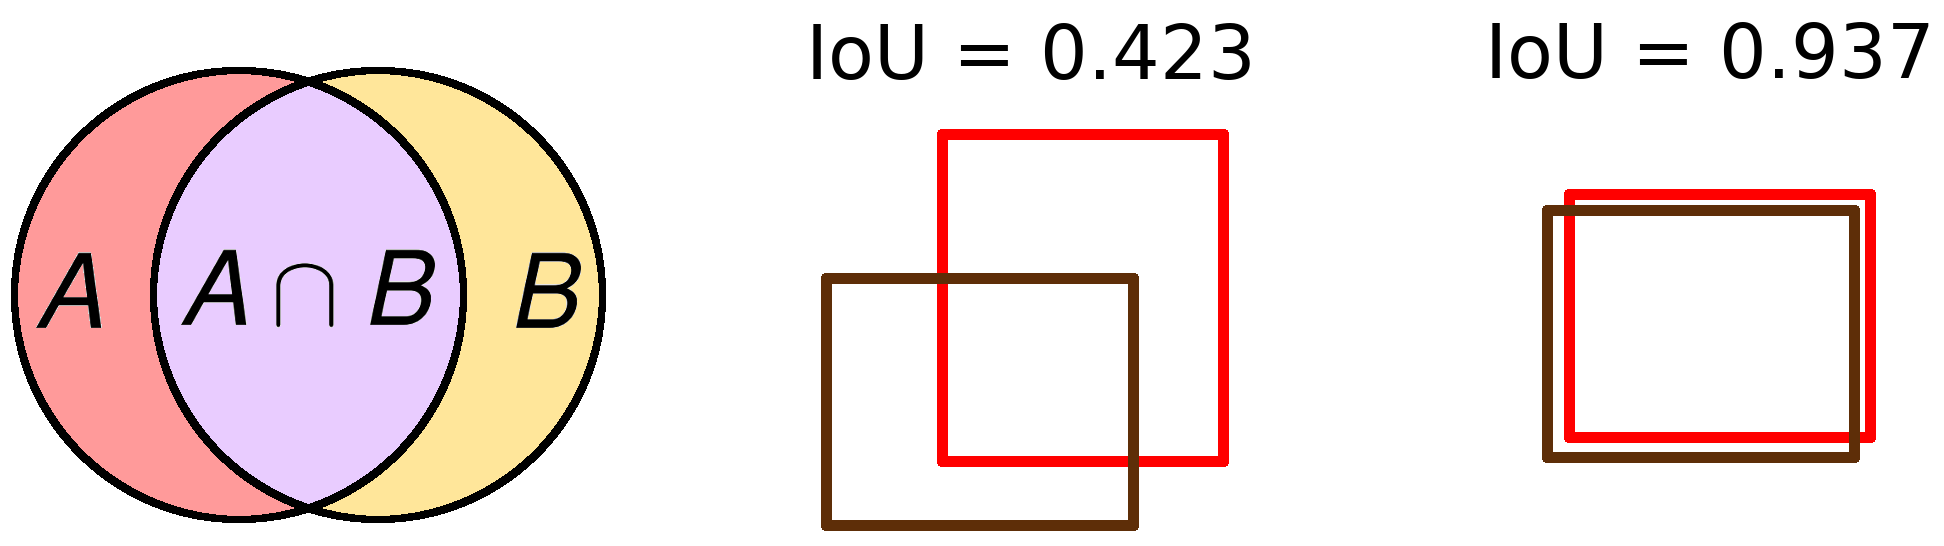
\includegraphics[width=10.6cm]{iou.png}
  \captionof{figure}{\footnotesize{IoU is defined as the size of the union divided by the size of the intersection of two sets $A$ and $B$.}} 
  \label{figiou}
\end{center}
\end{minipage}
\end{center}
\color{black!100}
Our FaceNet v1.0 baseline used the total loss function $L(\theta)$, which is the mean of the regression losses $L_r$ of all positively assigned anchors plus the mean of the classification losses $L_c$ of all anchors. Let $\hat{r}_a$ and $r_a$ be the predicted and ground truth coordinate offsets for anchor box $a$, and $\hat{p}_a$ and $p_a$ be the predicted and ground truth probability score respectively, for anchor $a$ to contain an object. Let $N$ be the set containing all anchor boxes $a$, and $N_{pos}$ be the set containing every positively assigned anchor box.
\begin{equation}\label{eqfacenetsoftmax}
L_r(x) = \begin{cases}
				0.5x^2 & \mbox{if } |x| < 1\\
				|x| - 0.5 & \mbox{otherwise}\\
			\end{cases}
\end{equation}
\begin{equation}\label{eqsmoothl1loss}
L_c(p, \hat{p}) = -p \log{\hat{p}}
\end{equation}
\begin{equation}
\begin{split}
	L(\theta) = &  \frac{1}{|N|} \sum_{a \in N} L_c(p_a, \hat{p}_a) 
	 + \frac{1}{|N_{pos}|} \sum_{a \in N_{pos}} L_r(r_a - \hat{r}_a)  \\ 
\end{split}
\end{equation}

All FaceNet versions were evaluated on the easy, medium, and hard splits of the WIDERFace dataset \cite{WIDERFace}, using the mean average precision (mAP) metric. It is defined as the integral of a model's precision $P(\theta)$ with respect to its recall $R(\theta)$.

\vspace{-14pt}

\begin{equation}
\textsf{mAP} = \int \limits^1_0 P(\theta) \hspace{4pt} \textsf{d}R(\theta) 
\end{equation}

\vspace{-6pt}

\end{posterbox}














\begin{posterbox}[name=zeropad,column=0,below=method, above=bottom]{Focal Loss versus Binary Cross Entropy}
Focal loss, used in RetinaNet \cite{retinanet}, introduced a loss function that focused on the training examples which were hard to classify. It was shown that using focal loss instead of cross entropy for multi-class object detection increased the final accuracy of the model. FaceNet v1.1 and v1.2 experimented using binary cross entropy $L_{BCE}$, and Focal Loss $L_{FL}$ respectively as their classification losses, defined as:

\begin{equation}
L_{BCE}(p, \hat{p}) = -p \log{(\hat{p})} -(1-p) \log{(1-\hat{p})}
\end{equation}

\begin{equation}
L_{FL}(p, \hat{p}) = -p (1-p)^\gamma \log{(\hat{p})} -(1-p) p^\gamma\log{(1-\hat{p})}
\end{equation}
\vspace{-3pt}

\begin{minipage}{0.57\linewidth}
   \centering
   \label{tabseqmnist}
   \scalebox{1}{
   \begin{tabular}{c c c c}
    \hline
    Model & mAP$_e$ & mAP$_m$ & mAP$_h$\\ \hline \hline
    v1.0 & 0 & 0 & 0 \\ \hline
    v1.1 & 37.4 & 21.7 & 9.7 \\ \hline
    v1.2 & 22.4 & 12.1 & 5.1  \\ \hline
    \end{tabular}}
\end{minipage}
\begin{minipage}{0.38\linewidth}
\captionof{table}{\footnotesize{\textbf{Versions 1.0 to 1.2}. Results on the easy (e), medium (m) and hard (m) WIDERFace splits.}}
\end{minipage}

\vspace{10pt}\color{black!100}
The baseline model, FaceNet v1.0, converged to predict a probability of zero that there existed an object for every bounding box. Later versions showed that Focal Loss performed considerably worse compared to binary cross entropy.
\end{posterbox}


















\begin{posterbox}[name=experiments,column=1, row=0]{Adding Feature Pyramids}
Our experiments showed that an addition of a Feature Pyramid Network (FPN) \cite{fpn} architecture leads to a dramatic increase in accuracy. FaceNet v1.3 and v1.4 used binary cross entropy and Focal Loss respectively with an FPN. Versions 1.5 and 1.6 experimented using a new pyramid-level-specific loss function $L(\theta)_{level}$. Here $L$ is the set of all pyramid levels $P$, and $N^P$ is the set of all created anchor boxes at every spatial position at pyramid level $P$:
\vspace{-6pt}
\begin{equation}
L(\theta)_{level} = \sum_{P \in L} \frac{1}{|N^P_{pos}|} ( \sum_{a \in N^P} L_c(p_a, \hat{p}_a) +  \sum_{a \in N^P_{pos}} L_r(r_a - \hat{r}_a) )
\end{equation}

\begin{minipage}{0.57\linewidth}
   \centering
   \label{tabseqmnist}
   \scalebox{1}{
   \begin{tabular}{c c c c}
    \hline
    Model & mAP$_e$ & mAP$_m$ & mAP$_h$\\ \hline \hline
    v1.3 & 89.3 & 85.9 & 65.9 \\ \hline
    v1.4 & 81.0 & 81.0 & 64.2 \\ \hline
    v1.5 & 87.2 & 82.5 & 50.4  \\ \hline
    v1.6 & 85.1 & 80.0 & 50.6  \\ \hline
    \end{tabular}}
\end{minipage}
\begin{minipage}{0.38\linewidth}
\captionof{table}{\footnotesize{\textbf{Versions 1.3 to 1.6}. Results on the easy (e), medium (m) and hard (m) WIDERFace splits.}}
\end{minipage}

\end{posterbox}



\begin{posterbox}[name=ohem,column=1,below=experiments]{Adding Online Hard Example Mining}
FaceNet v1.7 and v1.8 used Online Hard Example Mining (OHEM) \cite{ohem}, training on the top 128 classification losses, after non-maxima supression was applied. Version 1.7 applied OHEM separately on every example in the mini-batch, while version 1.8 used the whole mini-batch.

\begin{minipage}{0.57\linewidth}
   \centering
   \label{tabseqmnist}
   \scalebox{1}{
   \begin{tabular}{c c c c}
    \hline
    Model & mAP$_e$ & mAP$_m$ & mAP$_h$\\ \hline \hline
    v1.7 & 46.0 & 51.8 & 42.3 \\ \hline
    v1.8 & 55.9 & 36.8 & 15.6 \\ \hline
    \end{tabular}}
\end{minipage}
\begin{minipage}{0.38\linewidth}
\vspace{10pt}
\captionof{table}{\footnotesize{\textbf{Versions 1.7 and 1.8}. Results on the easy (e), medium (m) and hard (m) WIDERFace splits.}}
\end{minipage}
\vspace{-7pt}
\end{posterbox}








\begin{posterbox}[name=imagecaptioning,column=1,below=ohem]{New Features, Color Jitter, and Depth}
Versions 1.9 to 2.5 evaluated additional anchor box scales, IoU thresholds, deeper features, random color jitter and network depth. Most notable of these were the following versions: FaceNet v2.1 used features from \textit{conv3} to \textit{conv7} to increase computational speeds and to allow for deeper features. Bilinear interpolation was added to both sub-networks to offset the decrease in scale. Version 2.3 used additional data augmentation by randomly adding noise and shifting hues. To increase detection results on smaller faces, FaceNet v2.4 used anchors of sizes $8^2$ to $416^2$, and features from \textit{conv2} to \textit{conv7}.

%\vspace{10pt}
%A series of attempts were made, summarized by FaceNet v2.5, to increase network depth. ResNet-50 up to ResNet-151 \cite{resnet} were experimented on, as well as deeper sub-networks, but all attempts ended in the model converging to detect zero faces for every image.

\vspace{6pt}
\begin{minipage}{0.57\linewidth}
   \centering
   \label{tabseqmnist}
   \scalebox{1}{
   \begin{tabular}{c c c c}
    \hline
    Model & mAP$_e$ & mAP$_m$ & mAP$_h$\\ \hline \hline
    v2.1 & 89.1 & 86.6 & 64.4 \\ \hline
    v2.3 & 92.2 & 90.3 & 70.1 \\ \hline
    v2.4 & 89.6 & 86.8 & 75.8 \\ \hline
    \end{tabular}}
\end{minipage}
\vspace{4pt}
\begin{minipage}{0.38\linewidth}
\captionof{table}{\footnotesize{\textbf{Notable results from versions 1.9 to 2.5}. Results on the easy (e), medium (m) and hard (m) WIDERFace splits.}}
\end{minipage}

\end{posterbox}

















\begin{posterbox}[name=results,column=1,below=imagecaptioning]{Qualitative Results}


\begin{center}
\begin{minipage}{\textwidth}
\begin{center}
  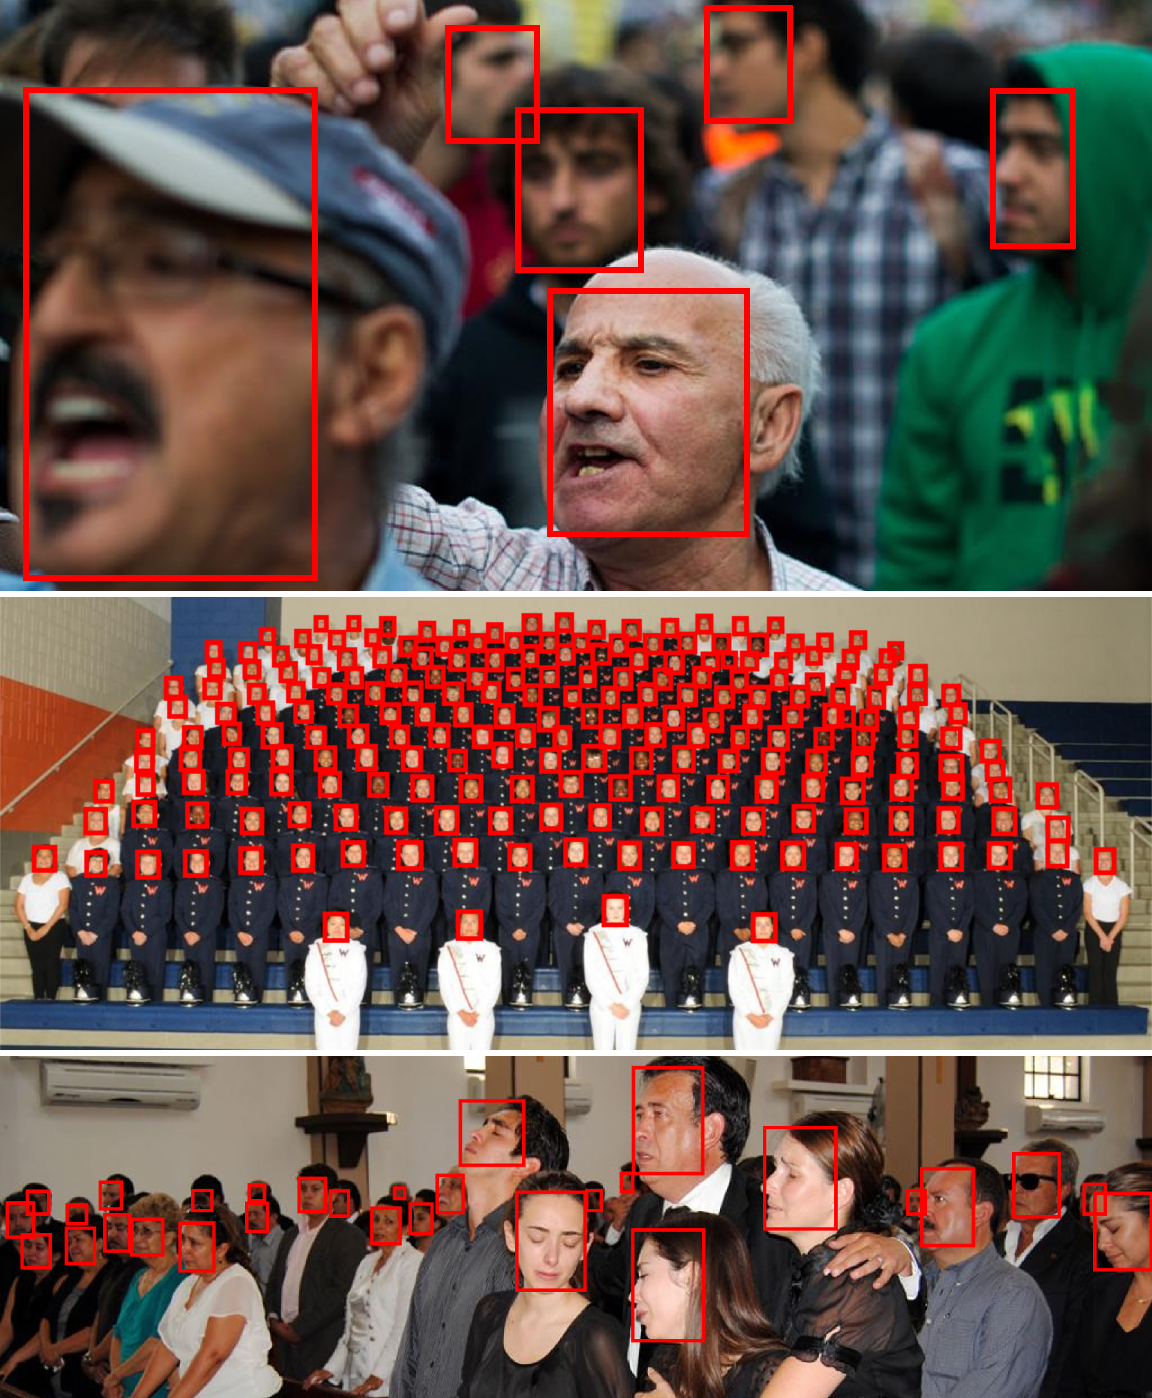
\includegraphics[width=11.5cm]{bigface3.png}
  \vspace{-15pt}
  \captionof{figure}{\footnotesize{Final results of FaceNet on the publically available WIDERFace \cite{WIDERFace} validation dataset.}} 
  \label{figimagecaptioning}
\end{center}
\end{minipage}
\end{center}

\end{posterbox}
















\begin{posterbox}[name=conclusion,column=1,below=results]{Conclusion}
Our final model is capable of dynamically detecting thousands of faces in a crowded scene for various scales, lighting and occlusions, with an inference time of 22 ms. In contrast to previous research, Focal Loss and Online Hard Example Mining was shown to decrease the accuracy of the object detector. The final model is sufficiently computationally efficient and accurate, achieving a mean average precision of 92.2, to serve as a baseline model for any system which incorporates surveillance, security or the detection of humans.
\end{posterbox}








\begin{posterbox}[name=references,column=1,below=conclusion, above=bottom, headerColorOne = blackcolor, headerColorTwo = blackcolor, borderColor = blackcolor]{References}
\vspace{-2pt}
All figures in this project were made by the project author Nikita Zozoulenko.
\bibliographystyle{plain}
\scalebox{0.65}{
\hspace{-10pt}
\begin{minipage}{{1.55\textwidth}}
\begin{thebibliography}{20}%
\itemsep=-0.01em% Save space between the separation
\setlength{\baselineskip}{0.4em}% Save space with longer lines
\bibitem{tcn} 
	\textit{An Empirical Evaluation of Generic Convolutional and Recurrent Networks for Sequence Modeling.}
	S. Bai, Z. Kolter, and V. Koltun
    arXiv preprint arXiv:1803.01271, 2018.
\bibitem{dilatedgru} 
	\textit{Dilated Recurrent Neural Networks.}
	S. Chang, Y. Zhang, W. Han, M. Yu, X. Guo, W. Tan, X. Cui, M. Witbrock, M. Hasegawa-Johnson, T. Huang
	arXiv preprint arXiv:1710.02224, 2017
\bibitem{mscoco}
	\textit{Microsoft COCO Captions: Data Collection and Evaluation Server.}
	X. Chen and H. Fang and TY Lin and R. Vedantam and S. Gupta and P. Dollár and C. L. Zitnick. 
	arXiv preprint arXiv:1504.00325, 2015
\bibitem{resnet} 
	\textit{Deep residual learning for image recognition.}
    K. He, X. Zhang, S. Ren, and J. Sun. 
    arXiv preprint arXiv:1512.03385, 2015.
\bibitem{yolo} 
	\textit{You only look once: Unified, real-time object detection.}
    J. Redmon, S. Divvala, R. Girshick, and A. Farhadi. 
    arXiv preprint arXiv:1506.02640, 2015.
\bibitem{ssd}
	\textit{{SSD:} Single Shot MultiBox Detector.}
	W. Liu and
               D. Anguelov and
               D. Erhan and
               C. Szegedy and
               S. Reed and
               C. Fu and
               A. Berg.
    arXiv preprint arXiv:1512.02325, 2015
\bibitem{yolo9000} 
	\textit{{YOLO9000:} Better, Faster, Stronger.}
    J. Redmon and
               A. Farhadi. 
    arXiv preprint arXiv:1612.08242, 2016.
\bibitem{dssd}
	\textit{{DSSD} : Deconvolutional Single Shot Detector.}
	C. Fu and
               W. Liu and
               A. Ranga and
               A. Tyagi and
               A. C. Berg
    arXiv preprint arXiv:1701.06659, 2017
\bibitem{retinanet}
	\textit{Focal Loss for Dense Object Detection.}
	Tsung{-}Yi Lin,
    Priya Goyal,
    Ross B. Girshick,
    Kaiming He and
    Piotr Doll{\'{a}}r.
    arXiv preprint arXiv:1708.02002, 2017
\bibitem{WIDERFace}
	\textit{WIDER FACE: A Face Detection Benchmark.}
	Yang, Shuo and Luo, Ping and Loy, Chen Change and Tang, Xiaoou
    IEEE Conference on Computer Vision and Pattern Recognition (CVPR), 2016
\bibitem{fpn}
	\textit{Feature Pyramid Networks for Object Detection.}
	Tsung{-}Yi Lin,
               Piotr Doll{\'{a}}r,
               Ross B. Girshick,
               Kaiming He,
               Bharath Hariharan and
               Serge J. Belongie.
    arXiv preprint arXiv:1612.03144, 2016
\bibitem{ohem}
	\textit{Training Region-based Object Detectors with Online Hard Example Mining.}
	A. Shrivastava, A. Gupta, and R. Girshick. 
	arXiv preprint arXiv:1604.03540, 2017

\end{thebibliography}
\end{minipage}}
\end{posterbox}











\end{poster}
\end{document}
